\documentclass[11pt]{article}
\usepackage[margin=1in]{geometry}
\usepackage{amsmath}
\usepackage{graphicx}
\usepackage{tikz-cd}
\usepackage{multicol}

\setlength{\parindent}{0pt}
\setlength{\parskip}{1\baselineskip}

\title{Climate regionalization of Serbia using Ant Colony Optimization}
\date{}

\begin{document}
\maketitle
\tableofcontents
\newpage

\section{Research motivation and objectives}
\label{sec:motivation}

\subsection{Motivation}

Climate regionalization is the process of dividing a geographical area into regions with similar climatic characteristics. Such regions are useful in many scientific and practical applications, including agriculture, forestry, ecology, hydrology, biodiversity conservation and spatial planning \cite{fovell1993,swenson2019}.

The most widely used climate regionalization is the Köppen-Geiger climate classification. It classifies climate using long-term temperature and precipitation statistics. It has been used for more than one hundred years. It is still common in climate studies and related fields \cite{koppen1936,peel2007,beck2018}.

Although the Köppen-Geiger classification is very successful as a global climate classification system, it was not designed to optimize regionalization for one country or one application. The classification is based on predefined climatic thresholds. These thresholds are applied worldwide \cite{koppen1936,peel2007}. Therefore, the system cannot adapt to local climatic characteristics or optimize the regions according to a chosen objective.

Recent work in climate regionalization often uses data-driven methods. In these methods, regions are formed from the data instead of fixed rules. Clustering is a common baseline because it groups locations with similar climate values \cite{fovell1993,carvalho2016}. Self-organizing maps are also used to find coherent climate and precipitation regions \cite{sheridan2011,swenson2019}. However, ordinary clustering can create fragmented maps. For this reason, spatial coherence is also important. ACO is useful here because it can search for region assignments while combining more than one criterion \cite{dorigo1996,dorigo2004}.

The goal of this work is not to replace the Köppen-Geiger classification as a universal climate classification system. Instead, the objective is to investigate whether a data-driven optimization approach can produce a regionalization that is better suited for Serbia while using comparable climatic information.

In the proposed approach, each ant constructs one candidate climate regionalization. One ant assigns every spatial unit to one of a predefined number of climate regions. A complete ant solution is therefore a vector of cluster labels, with one label assigned to each spatial unit. The quality of each candidate regionalization is evaluated using one of several fitness functions. Each fitness function defines a different view of what a good regionalization means. Ant Colony Optimization then searches for the assignment that minimizes the selected fitness function.


\subsection{Research objectives}
The main objective of this research is to develop an optimization framework for climate regionalization based on Ant Colony Optimization (ACO).
The current result is not a single optimized climate map, but an optimization framework that allows comparing different strategies. At this point, this work includes:

\begin{itemize}
    \item preprocessing pipeline for transforming climatic raster data into a format suitable for optimization
    \item a couple of ACO construction strategies and heuristic functions
    \item comparison of different fitness functions
    \item investigation of different pheromone update strategies and algorithm parameters
    \item comparison of the proposed approaches with the KMeans as a baseline
    \item comparison of the new classification with the Köppen-Geiger regionalization
    \item external validation measures based on independent land cover information, inspired by the original purpose of Koppen regionalization
\end{itemize}


\section{Köppen-Geiger climate classification}
\label{sec:koppen}

\subsection{Historical background}

The Köppen-Geiger climate classification is one of the oldest and most widely used climate classification systems. It was originally developed by Wladimir Köppen. It was later refined together with Rudolf Geiger \cite{koppen1936,peel2007}. During the following decades the classification became a common reference for describing climate regions throughout the world \cite{peel2007,beck2018}.

The original motivation behind the Köppen classification was to describe the relationship between climate and natural vegetation \cite{koppen1936,peel2007}. Köppen observed that regions with similar temperature and precipitation conditions often support similar types of vegetation. He therefore designed the classification so that climate zones would approximately correspond to the major vegetation regions of the world.

Unlike many regional climate classifications developed for specific countries, the Köppen-Geiger system was designed as a global classification. The same classification rules are applied to every location. Because of its simplicity, reproducibility and long history, it is still widely used in climatology, ecology, agriculture, forestry and other environmental sciences \cite{peel2007,beck2018}.

The classification has also been updated several times using newer climatic observations. These updates preserve the original classification principles \cite{peel2007,beck2018}. This has allowed the system to remain relevant despite changes in the global climate.

The Köppen-Geiger classification has also been applied directly to Serbia. Milovanović et al. \cite{milovanovic2017} used temperature and precipitation data to map Köppen climate types in Serbia. This makes it a useful local reference for this study.

\subsection{Climate classes}

The classification is hierarchical. The class labels consist of three letters. The first level of the Köppen-Geiger classification divides the world's climates into five major climate groups \cite{koppen1936,peel2007}.

\begin{table}[h]
\centering
\begin{tabular}{ll}
\hline
Group & Description \\
\hline
A & Tropical climates \\
B & Arid climates \\
C & Temperate climates \\
D & Continental climates \\
E & Polar climates \\
\hline
\end{tabular}
\caption{Main Köppen-Geiger climate groups.}
\end{table}

Additional letters provide more detailed information about the climatic conditions. The second letter usually describes the precipitation regime, for example whether precipitation is evenly distributed throughout the year or concentrated in particular seasons. The third letter describes the thermal characteristics of the climate, such as summer temperature or winter severity. Combining these letters produces climate classes such as Cfa, Cfb, Dfb, etc.

Although the complete Köppen-Geiger system contains many different climate classes, only a small subset is present within Serbia. These classes will be introduced together with the Köppen reference dataset used later in this work.

\subsection{Advantages}

The Köppen-Geiger classification has remained widely used for more than one hundred years for several reasons \cite{peel2007,beck2018}.

\begin{itemize}
    \item It is simple and easy to interpret.
    \item It is based on physically meaningful climatic variables.
    \item The same methodology can be applied worldwide.
    \item The resulting climate classes are reproducible.
    \item The classes have a strong relationship with natural vegetation.
    \item It provides a common reference used across many scientific disciplines.
\end{itemize}

These characteristics make the Köppen-Geiger classification an appropriate reference when evaluating alternative climate regionalization methods \cite{peel2007,beck2018}.

\subsection{Limitations}

Despite its widespread use, the Köppen-Geiger classification also has several limitations when used for regional climate regionalization \cite{fovell1993,swenson2019}.
\begin{itemize}
  \item The classification is entirely rule-based. Every location is assigned to a climate class using predefined thresholds instead of optimizing the resulting regions according to a specific objective.
  \item The boundaries between climate classes are determined by fixed threshold values. Small differences in temperature or precipitation around these thresholds may result in different climate classes even though the climatic conditions are very similar.
  \item Depending on the granularity of the map, rule-based classification might result in inconvinient small clusters, which can make the regionalization look fragmented and incoherent
\end{itemize}

The objective of this research is therefore not to replace the Köppen-Geiger classification as a universal climate classification system. Instead, it is used as a well-established reference against which the proposed optimization-based regionalization can be compared.

These limitations are one reason why data-driven regionalization methods are also used in climate studies. Cluster analysis has been used to define climate regions from temperature and precipitation data \cite{fovell1993}. KMeans has been used for climate-change regionalization in Europe \cite{carvalho2016}. Self-organizing maps are another common approach for finding coherent climate or precipitation regions \cite{sheridan2011,swenson2019}. This work follows the same general idea. It forms regions from data. However, it uses ACO instead of a standard clustering algorithm.



\section{Data preparation: climate raster files and final dataframe}
\label{sec:data-prep}

\subsection{Short summary}
The first step was to prepare the climate data in a form that can be used for clustering. The input data consisted of several .tif raster files, where each file represents one climate variable over Serbia. Since the rasters had to be used together, they were first put onto the same spatial grid. After that, the value from every raster was extracted for every grid cell and stored in one table. Rows with missing values were removed, so the final dataframe contains only locations where all climate variables are available. This final table is saved as df\_valid.csv and is used as the input for the later preprocessing and clustering pipeline.

This removed 252,145 cells, or 45.55\% of the rectangular raster grid. Most of these cells were outside the study-area mask. This was checked against the GADM Serbia boundary \cite{gadm2022}. Only 3,001 removed cells were inside the GADM polygon. Some valid cells were outside the GADM polygon because the climate raster includes Kosovo, while the GADM Serbia boundary used here does not.

Key input \& outputs:
\begin{verbatim}
  Inputs:
  - Climate raster layers (.tif)

  Outputs:
  - master_df.csv
  - df_valid.csv

  Used later by:
  - preprocessing.py
\end{verbatim}

\subsection{Detailed explanation}
The climate data used in this work were obtained from the Serbian Academy of Science and Art (SANU). The dataset consists of raster maps representing long-term climatic averages over the territory of Serbia. The rasters contain monthly, seasonal and annual summaries of temperature and precipitation. 
The climate dataset consists of 31 raster layers. The layers include monthly, seasonal and annual averages of air temperature (1961–2010) and monthly, seasonal and annual precipitation totals. These layers are continuous raster variables, such as temperature or precipitation values for different seasons or annual summaries.

\begin{table}[ht]
  \centering
  \label{tab:climate_layers}
  \begin{tabular}{lr}
    \textbf{Variable type} & \textbf{Number of layers} \\
      Monthly temperature      & 12 \\
      Seasonal temperature     & 4  \\
      Annual temperature       & 1  \\
      Monthly precipitation    & 9  \\
      Seasonal precipitation   & 4  \\
      Annual precipitation     & 1  \\
    \textbf{Total}           & \textbf{31} \\
  \end{tabular}
  \caption{Climate raster layers used to construct the final dataset.}
\end{table}


Monthly precipitation rasters were available for only nine months. The initial data are stored as multiple GeoTIFF files in the folder Karte. Each .tif file contains one climate-related layer. Because the goal is to compare all climate variables at the same spatial locations, all rasters first need to have the same grid. This means they need to have the same:

\begin{itemize}
  \item coordinate reference system
  \item spatial resolution
  \item raster width and height
\end{itemize}

In this stage, one raster is used as the reference raster. All other rasters are then resampled and reprojected so that they match this reference grid. The aligned rasters are saved into a new folder called Karte\_jedna\_mreza. After this step, all climate layers have the same shape and can be safely combined cell by cell.

The next step is to create one table from the aligned rasters. For each raster cell, the notebook records:

\begin{itemize}
  \item row
  \item col
  \item easting
  \item northing
\end{itemize}

The row and col columns identify the position of the pixel within the raster grid. They are later used to reconstruct raster maps from the dataframe and to merge the climate data with external datasets such as vegetation and the Köppen-Geiger classification.The easting and northing values describe the real projected UTM coordinates of each raster cell.

Then, for every climate raster, a new column is added to the dataframe. Each row therefore represents one spatial cell/pixel, and each climate column gives the value of one climate variable at that location.

At the end, rows with missing values are removed. This is important because some raster cells may fall outside the valid area (Serbia), or some variables may not have values at all locations. The final dataframe keeps only rows where all climate variables are available.

The notebook reports:
\begin{verbatim}
  Total cells: 553 539
  Valid cells after removing missing values: 301 394
  Number of climate columns: 31
\end{verbatim}

The final output is saved as: \texttt{df\_valid.csv}. This file is the main input for the next stages of the project. It contains the spatial coordinates and all climate variables for the valid grid cells.


\section{Preprocessing}
\label{sec:preprocessing}

\subsection{Short summary} 
The purpose of the preprocessing module is to transform the climate dataframe into a representation that can be directly used by the clustering algorithms. Besides selecting the input features, the module also creates the spatial neighborhood graph, optionally groups pixels into superpixels, standardizes the feature values and returns all information required by the optimization algorithms. The output of this module is the common input format used by all clustering methods.

\subsection{Detailed explanation}
\subsubsection{Common preprocessing pipeline}

All clustering algorithms use the same preprocessing pipeline. This ensures that differences in the final results come from the optimization algorithm itself rather than from differences in the input data.

The preprocessing module receives the dataframe created in the previous step (df\_valid.csv) and produces a standardized representation consisting of:
\begin{itemize}
  \item feature matrix (X\_model)
  \item spatial coordinates of every node
  \item node weights
  \item neighborhood graph
  \item mapping between original pixels and optimization nodes
\end{itemize}

Depending on the selected mode, one optimization node may represent either a single pixel or an aggregated superpixel

\subsubsection{Feature construction}
One of the goals of the project is to investigate how different feature representations affect the quality of climate regionalization. For this reason the preprocessing module supports three different feature sets.

\textbf{Raw climate variables} \\
The simplest representation uses all climate variables directly. Every raster layer becomes one feature, resulting in a feature vector containing all available temperature and precipitation variables. This representation preserves all available information but also contains a large number of correlated variables. In the later experiments this representation is used together with the Köppen-inspired and PCA representations in order to test whether the conclusions depend on feature construction.

\textbf{Köppen-inspired features} \\
Instead of using all climate variables directly, the second option constructs a smaller set of summary statistics inspired by the Köppen climate classification. The following quantities are computed separately for every spatial location:

\begin{itemize}
  \item mean temperature
  \item minimum temperature
  \item maximum temperature
  \item temperature range
  \item mean precipitation
  \item minimum precipitation
  \item maximum precipitation
  \item total precipitation
  \item precipitation range
\end{itemize}

Additional optional variables such as temperature standard deviation, precipitation standard deviation and a simple dryness index are also implemented, although they were not used in the current experiments. This mode was the initial feature representation and is used as the main reference feature set in the report.

\textbf{PCA features} \\
The third option applies Principal Component Analysis separately to temperature and precipitation variables. Instead of combining all variables into a single PCA model, the two groups are transformed independently, producing separate principal components for temperature and precipitation. This preserves the distinction between the two climate components while still reducing dimensionality. This representation was evaluated using the same Stage 1 sweep and Stage 2 validation protocol as the other feature representations.

\subsubsection{Superpixel generation}
The preprocessing module supports two optimization modes. In pixel mode, every original raster cell becomes one optimization node. In superpixel mode, neighboring pixels are first grouped into larger spatial units using MiniBatch K-Means applied only to spatial coordinates. The average climate values of all pixels belonging to one superpixel become the feature vector of the new optimization node. Since every graph node represents a different number of original raster cells, the size of each superpixel is stored as a node weight, allowing larger regions to contribute proportionally during optimization, when cluster centroids and fitness values are calculated. 

\subsubsection{Feature scaling}
Because climate variables have different numerical ranges, the feature values are standardized before clustering. The module uses standardization after the final feature representation has been constructed. This prevents variables with larger numerical ranges from dominating the distance calculations used by the optimization algorithms.

\subsubsection{Neighborhood graph}
After the optimization nodes have been created, a spatial neighborhood graph is constructed using the k-nearest-neighbor algorithm on the row and column features. This graph is later used by several heuristic functions and by the spatial component of the objective function. The number of neighbors is configurable, allowing experiments with different neighborhood sizes.

\subsubsection{Final model representation}
The last function of the module combines all preprocessing steps into a single pipeline. Depending on the selected configuration, it:
\begin{itemize}
  \item builds the chosen feature representation
  \item optionally creates superpixels
  \item standardizes the feature values
  \item constructs the neighborhood graph
  \item returns all information required by the clustering algorithms
\end{itemize}
The resulting structure is then passed unchanged to all optimization algorithms implemented later in the project.


\section{Ant clustering engine, fitness functions and pheromone updates}
\label{sec:frameworsk}

\subsection{Short summary}
This part of the code defines the main optimization framework. The goal was to make one common engine that can run different ant-based clustering strategies under the same conditions. The engine does not decide how one ant builds a clustering solution. Instead, that part is passed in as a separate construction function. After each ant builds a solution, the solution is evaluated using one of the tested fitness functions and pheromone values are updated.

The method is related to earlier work on ant-based clustering and topographic mapping \cite{deneubourg1991,handl2006}. Those studies show how simple ant-like agents can be used to form groups from data. This work uses the same general idea, but applies it to climate regionalization. The focus is on comparing construction strategies for spatial climate regions, rather than on reproducing a standard ant-based clustering algorithm.

ACO has also been used in spatial environmental optimization. Examples include protected-area zoning, ecological corridor detection, land-use optimization and urban heat mitigation \cite{liu2012,peng2019,zhang2021,tong2024}. These studies are not climate regionalization studies. However, they show that ACO can be useful for spatial problems with ecological or compactness objectives.

The experiments use three fitness functions. Each fitness function defines a different view of what a good regionalization means. The centroid-based fitness favors compact groups in feature space. The silhouette-based fitness compares cohesion and separation. The graph-based fitness emphasizes local similarity on the spatial neighborhood graph. All three fitness functions are tested on the same parameter grid.

The pheromone matrix stores a learned preference for assigning each node to each cluster.


\subsection{Detailed explanation}

\subsubsection{Main optimization engine}
The main optimizer is implemented in AntClusteringOptimizer. Its role is to control the general ant-colony optimization loop.

The optimizer is intentionally generic. It does not contain the actual solution construction logic. Instead, it receives several functions as input:
\begin{itemize}
  \item construct\_solution\_fn
  \item fitness\_fn
  \item pheromone\_update\_fn
  \item pheromone\_init\_fn
\end{itemize}
This means that different clustering strategies can be compared fairly. The outer optimization loop stays the same, while only the construction strategy changes.

In each iteration, the optimizer runs several ants. Each ant constructs one complete clustering solution. A solution consists of:
\begin{itemize}
  \item labels
  \item centroids
\end{itemize}
The labels array contains the assigned cluster for every node. The centroids array contains the cluster centers computed from that assignment.

After a solution is constructed, it is evaluated by the fitness function. For every ant, the optimizer stores:
\begin{itemize}
  \item fitness
  \item labels
  \item centroids
  \item fitness terms
\end{itemize}

The best solution found so far is kept during the full optimization process. At the end, the optimizer stores the final best result in:
\begin{itemize}
  \item labels\_
  \item centroids\_
  \item best\_fitness\_
  \item history\_
  \item term\_history\_
  \item pheromone\_
\end{itemize}

The history\_ list stores the global best fitness after every iteration. The term\_history\_ list stores more detailed information, including iteration-best fitness, mean fitness, standard deviation, compactness, spatial disagreement and pheromone minimum/maximum values.

\subsubsection{Pheromone matrix}
The pheromone matrix has shape:
\texttt{number of nodes × number of clusters}.
Each value means:
\texttt{pheromone[i, k] = learned preference for assigning node i to cluster k}. 
At the beginning, all node-cluster assignments have equal pheromone values. If row normalization is used, each row sums to 1. This representation is appropriate for clustering because the final decision for every node is exactly the choice of one cluster label. \texttt{number of clusters} is 5 based on the number of major Köppen classes present in Serbia.

\subsubsection{General optimization loop}
The optimization process can be summarized as:
\begin{verbatim}
initialize pheromone
for each iteration:
    for each ant:
        construct a clustering solution
        evaluate the solution
        store the solution
    update pheromone
    update global best solution
    save iteration statistics
\end{verbatim}

The implementation also allows pheromone updates after smaller batches of ants. If no batch size is given, pheromone is updated once after all ants in the iteration. If a batch size is given, pheromone is updated several times inside the same iteration. This was useful during experimentation because it made it possible to compare iteration-level, colony-level, batch-level, and ant-level learning behavior.

\subsubsection{Fitness functions}
The experiments use three fitness functions. They define three different optimization objectives. Lower values are better in all three cases.

\textbf{Centroid-based fitness} \\
The centroid-based fitness function is a weighted sum of two terms:
\begin{verbatim}
fitness =
    w_compactness * compactness
  + w_spatial * spatial_disagreement
\end{verbatim}

The first term is feature compactness. It measures how close nodes are to the centroid of their assigned cluster. This is normalized by the total variance of the data, so the value is easier to compare across different feature representations. All centroid and variance calculations are weighted using the superpixel node weights described in the preprocessing stage. This ensures that the optimization approximates the result that would be obtained if the algorithm operated directly on the original raster cells.
The second term is spatial disagreement. It measures the fraction of neighboring node pairs that have different cluster labels. If many neighboring nodes belong to different clusters, the map is fragmented and spatial disagreement is high. If neighboring nodes often belong to the same cluster, spatial disagreement is low.

The default weights used in the experiments were:
\begin{verbatim}
  w_compactness = 0.7
  w_spatial = 0.3
\end{verbatim}

This means that the objective gives more importance to feature compactness, while still encouraging spatially smoother clusters. 

\textbf{Silhouette-based fitness} \\
The silhouette-based fitness uses the silhouette score instead of centroid compactness. For each node, it compares two distances. The first distance is the average distance to nodes in the same cluster. The second distance is the average distance to the nearest other cluster. A high silhouette score means that a node is closer to its own cluster than to other clusters.

Since the optimizer minimizes fitness, the silhouette score is converted into a minimization term:
\begin{verbatim}
silhouette_term = (1 - mean_silhouette) / 2
\end{verbatim}

The final fitness is:
\begin{verbatim}
fitness =
    w_silhouette * silhouette_term
  + w_spatial * spatial_disagreement
\end{verbatim}

\textbf{SNN-based fitness} \\
The SNN-based fitness uses a shared-nearest-neighbor graph. This graph connects nodes that have similar local neighborhoods in feature space. The fitness measures how much of this graph is cut by the clustering. If many strong SNN links connect nodes with different labels, the SNN cut is high.

The final fitness is:
\begin{verbatim}
fitness =
    w_snn * snn_cut
  + w_spatial * spatial_disagreement
\end{verbatim}

This objective does not use cluster centroids in its main term. It therefore defines regionalization quality differently from the centroid-based fitness.


\subsubsection{Compactness}
Compactness is computed as:
\texttt{within-cluster variance / total variance}. The numerator measures how far each node is from the centroid of its assigned cluster. The denominator measures the total variance of the full dataset around the global centroid. This normalization makes the compactness term dimensionless. That is useful because experiments may use different feature sets, such as raw climate variables, PCA features, or Köppen-inspired features.

One important note is that this compactness term is centroid-based. Therefore, even if a construction strategy uses a non-centroid heuristic, the final fitness still partly rewards centroid-like cluster structure. This is not an implementation error, but it is important for interpreting the results.

\subsubsection{Spatial disagreement}
Spatial disagreement uses the neighborhood graph created during preprocessing. For each node, the function checks its neighbors. If a neighbor has a different label, this counts as a disagreement. The final score is:
\texttt{number of disagreeing neighbor links / total number of neighbor links}. The value is between 0 and 1. A value close to 0 means neighboring nodes usually belong to the same cluster. A larger value means the clustering is more fragmented.

The function supports two modes:
\begin{enumerate}
  \item directed neighbor counting;
  \item symmetric neighbor counting.
\end{enumerate}

In the current experiments, the directed version was used because it directly matches the k-nearest-neighbor graph produced by preprocessing.


\subsubsection{Pheromone update strategies}
Three pheromone update strategies were implemented.

\textbf{All-ants update} \\
This strategy uses information from the whole ant population, not only the best solution. In this strategy, every ant deposits pheromone after evaporation. Since lower fitness is better, lower fitness produces a larger deposit. Better solutions deposit more pheromone because the deposit is computed as:
\texttt{q / fitness}

\textbf{Best-ant update} \\
In this strategy, only the best ant from the current batch deposits pheromone. This is more exploitative than the all-ants update. It pushes the search more strongly toward the best solution found in the current batch, but it can also reduce diversity more quickly.

\textbf{Quality-weighted update} \\
In this strategy, deposit is based on how much better each solution is than the average solution in the current batch. Solutions worse than or close to the average receive little or no pheromone. The best solution receives the strongest reinforcement. This strategy was added to make pheromone deposition depend on relative solution quality, not only on absolute fitness.


\subsubsection{Current implementation}
This part of the implementation is relatively stable. The optimizer, fitness functions, and pheromone update functions form the common experimental framework. They are not specific to one heuristic or one construction strategy.

The choice of fitness function affects how the results should be interpreted. The centroid-based fitness rewards centroid compactness, so it may favor KMeans-like solutions. The other fitness functions define regionalization quality differently. This makes it possible to compare construction strategies under different optimization objectives.

\section{Construction strategies and heuristics}
\label{sec:strategies}

\subsection{Short summary}
This part of the code defines how a single ant builds one clustering solution. The optimizer described in the previous section controls the outer loop, but it does not decide how labels are assigned. That decision is handled by the construction strategies.

Each construction strategy assigns every node to one of the available clusters. The assignment probability depends on two parts: the pheromone value learned from previous ants and a heuristic score computed from the current partial solution. Several heuristics were tested, including centroid similarity, graph-local similarity, cohesion similarity and spatial support.

The purpose of this part of the project was to test different ways of constructing climate regions, especially alternatives that are less directly tied to KMeans-style centroid compactness.

\subsection{Detailed explanation}

\subsubsection{Role of construction strategies}
A construction strategy defines how one ant creates a complete clustering solution. At the beginning of construction, all nodes are unassigned. The ant then visits nodes in random order. For each node, it computes a probability of assigning that node to each cluster. The node is then assigned by sampling from this probability distribution. After all nodes have been assigned, the centroids are recomputed and the complete solution is returned to the optimizer.

In general, the probability depends on: \texttt{pheromone score × heuristic score}. The pheromone score comes from previous iterations and represents learned preference. The heuristic score is computed from the current partial solution and depends on the selected construction strategy.

\paragraph{Initialization}

Before solution construction begins, all spatial units are marked as unassigned by setting their cluster labels to $-1$. The initialization of cluster centroids depends on the selected construction strategy.

For the centroid-based ACO and ACO Refinement strategies, all centroids are initially set to zero and are updated as nodes are assigned to clusters.

Graph-based strategies require centroid estimates before enough neighboring nodes have been assigned. Therefore, the initial centroids are generated using the KMeans++ initialization procedure. 

\subsubsection{Basic ACO construction}

The basic ACO construction strategy builds one solution in a single pass. It visits all nodes once in random order and assigns each node to a cluster.

The construction procedure is independent of the heuristic used. In the centroid-based variant, the heuristic score is computed from the distance between the current node and the temporary centroid of each cluster. In the cohesion-based variant, the heuristic is based on the similarity between the current node and the nodes that have already been assigned to each cluster. 


\subsubsection{ACO with refinement}

The refinement strategy extends the single-pass construction. After the initial solution has been constructed, cluster centroids are recomputed and the nodes are reassigned. This process is repeated several times, allowing the solution to improve after the initial construction pass.

The refinement procedure consists of the following steps:

\begin{enumerate}
    \item assign cluster labels,
    \item recompute cluster centroids,
    \item reassign cluster labels,
    \item recompute cluster centroids,
    \item repeat for the specified number of refinement iterations.
\end{enumerate}

As with the basic ACO strategy, the refinement procedure can be combined with either the centroid-based or the cohesion-based heuristic. The refinement mechanism itself is independent of the heuristic used for node assignment.


\subsubsection{Graph-local construction}
The graph-local construction strategy uses the spatial neighborhood graph during assignment. For a node currently being assigned, the algorithm checks which of its neighboring nodes have already received labels. It then compares the node’s feature vector with the feature vectors of already assigned neighbors in each candidate cluster. If a node is similar to neighboring nodes that already belong to cluster k, then cluster k receives a higher heuristic score.

However, this heuristic also contains a centroid fallback. When few neighboring nodes have already been assigned, the local graph evidence is weak. In that case, the heuristic partly relies on distance to initialized centroids.

So this strategy is not purely graph-based. It is better described as: \texttt{local graph similarity with centroid fallback}.


\subsubsection{Multi-colony construction}
The multi-colony strategy was introduced to allow different types of ants to use different heuristics while sharing the same pheromone matrix. In this strategy, ants are divided into colonies. Each colony has its own heuristic function. For example, one colony may use a centroid heuristic, another may use a graph heuristic, and another may use a spatial heuristic. This was added to test whether combining several types of local decision rules could produce better clustering than relying on a single heuristic.

The colony assignment is currently done sequentially by ant index. If there are three colonies and fifteen ants, the first group of ants belongs to the first colony, the second group to the second colony, and the last group to the third colony.

All colonies still write to the same pheromone matrix. This means that different search behaviors can contribute to the same learned assignment preferences.



\subsubsection{Heuristics}

\textbf{Centroid heuristic} \\
The centroid heuristic assigns higher probability to clusters whose current centroid is close to the node being assigned. This heuristic is closest to the logic of KMeans, although the assignment is still stochastic and influenced by pheromone.

For each candidate cluster, the squared distance between the node and the centroid is computed. Smaller distance gives a larger score.


\textbf{Graph-local heuristic} \\
The graph-local heuristic uses already assigned spatial neighbors. For each candidate cluster, it checks whether any assigned neighbors already belong to that cluster. If they do, the feature distance between the current node and those neighbors is computed. Smaller average distance gives a larger score.

Because early in the construction process many neighbors may still be unassigned, this heuristic blends the graph score with a centroid score. The more assigned neighbors are available, the more the graph score matters.


\textbf{Spatial heuristic} \\
The spatial heuristic uses only labels of already assigned neighbors. It does not use feature distances or centroids. If many assigned neighbors already belong to a certain cluster, that cluster receives a higher score.

This heuristic was introduced to encourage spatially smoother and less fragmented cluster maps. It's never used on its own, just in multi-heuristic strategies.


\textbf{Cohesion heuristic} \\
The graph-cohesion heuristic was introduced as an alternative to centroid-based assignment. Instead of asking \texttt{Is this node close to the cluster centroid?} it asks: \texttt{Is this node similar to existing members of this cluster?}. This heuristic is useful because it reduces direct dependence on centroids and can represent cluster cohesion in a less KMeans-like way.

For each candidate cluster, the heuristic samples already assigned members of that cluster and computes the average feature distance between them and the current node. Smaller average distance gives a higher score.

To avoid unstable behavior when clusters are still too small, the heuristic only uses a cluster if it already has more than a minimum number of assigned members. In the current code, that threshold is 15 members and the maximum sample size is 40.


\subsection{Current state of this part of the code}
This module contains the most experimental part of the project. It includes several construction strategies and heuristics that were introduced while testing different ways to move beyond simple centroid-based clustering. 

There are  two choices that are intentional and should be documented rather than treated as errors.
\begin{enumerate}
  \item The graph-local heuristic includes a centroid fallback. This was added because, early in construction, many spatial neighbors are still unassigned. In that situation, a purely graph-based score has little information. The centroid fallback gives the heuristic a weak feature-based signal until enough neighboring labels are available.
  \item The multi-colony strategy includes a small mutation mechanism. The goal of this mutation is not to target one specific colony, but only to affect a small subset of ants. This keeps some exploration in the search process without randomizing all ants or all colonies. In the current implementation, the mutation parameters are hardcoded, but they could later be made configurable.
\end{enumerate}

Overall, the construction and heuristic module should be understood as the experimental part of the method. It contains the main alternatives that were tested: centroid-based construction, graph-local construction, cohesion-based construction, refinement, and multi-colony construction. The final experiments will determine which of these variants should remain in the final comparison.



\section{Validation methodology}
\label{sec:validation}

\subsection{Internal optimization measure}
The optimization process is guided by the fitness function defined in Section 3. The fitness value is reported for every experiment as the internal optimization measure. Since the fitness function is directly optimized by the algorithm, it is not sufficient as an independent evaluation criterion.


\subsection{External ecological validation}
\subsubsection{Motivation}
Different climate conditions are associated with different types of land cover. Forests, shrublands, grasslands and other natural land cover types develop under different climatic conditions. Therefore, consistent land cover segregation within climate regions may indicate that the obtained regionalization captures at least part of the underlying climate variability. This section describes the proposed ecological consistency metric together with the dataset used for its calculation.


\subsubsection{Land cover categorization by climate influence}
Natural vegetation develops under long-term climatic conditions. Areas with similar climate are expected to have similar natural vegetation.

Agricultural areas are different. Climate is still an important factor, but land management, farming practices and economic decisions also influence land cover. Because of this, agricultural areas should not be treated in the same way as natural vegetation.

Artificial areas are even less suitable for climate validation. Urban development and infrastructure depend mainly on human decisions. They therefore provide little information about climate regionalization.

For these reasons, the proposed validation method evaluates agricultural and natural areas separately. Artificial areas are excluded from the final score.

This approach allows every climate region to be evaluated using the land cover types that are most informative for that part of the landscape.


\subsubsection{CORINE Land Cover dataset}
The external validation is based on the CORINE Land Cover (CLC) 2018 dataset produced by the Copernicus Land Monitoring Service \cite{copernicusCLC2018,clcManual2021}.

The raster version with a spatial resolution of 100 m was used in this work. Every raster cell belongs to one of the official CLC land cover classes. The dataset covers the entire territory of Serbia and was reprojected to match the coordinate reference system used by the climate dataset.

The vegetation dataset is completely independent of the climate variables used during clustering. It is therefore suitable for evaluating whether the obtained climate regions correspond to meaningful environmental regions.

The original CLC dataset contains many detailed land cover classes. For the purpose of validation, these classes were grouped into broader categories.

The following natural categories were used:
\begin{itemize}
  \item Broadleaf forest
  \item Coniferous forest
  \item Mixed forest
  \item Shrubland
  \item Grassland and bare land
  \item Wetlands
  \item Water
\end{itemize}

Areas that had one of the agricultural classes were kept as a separate category. Unlike natural vegetation, agricultural land is strongly influenced by human management. However, different agricultural land cover classes still provide useful information about climate suitability.

Artificial surfaces were also identified separately. These areas mainly represent cities, roads and other built-up infrastructure. Their spatial distribution is determined mostly by human activity rather than climate. Artificial areas are therefore excluded from the ecological consistency score. Their proportion is still reported as additional information.

\subsubsection{Ecological consistency of agricultural areas}
Shannon entropy was selected for measuring area consistency because it measures the diversity of land cover classes within a climate region. Lower entropy indicates that most pixels belong to a small number of land cover classes, while higher entropy indicates a more heterogeneous region.

For every climate region, only pixels classified as agricultural land are selected. The relative proportion of every agricultural land cover class is calculated. Let $p_i$ represent the proportion of agricultural class $i$, where
\[
\sum_{i=1}^{m} p_i = 1.
\]

The Shannon entropy is
\[
H_A=-\sum_{i=1}^{m} p_i \log(p_i).
\]
Since different clusters may contain different numbers of agricultural classes, the entropy is normalized.
\[
H_A^{\mathrm{norm}}
=
\frac{H_A}{\log(m)}.
\]
The agricultural consistency is then defined as
\[
G_A
=
1-H_A^{\mathrm{norm}}.
\]
The value of $G_A$ is between 0 and 1. A value close to 1 indicates that most agricultural land belongs to only a few land cover classes. This means that the agricultural areas inside the climate region are relatively homogeneous. Lower values indicate a more diverse agricultural structure.

\subsubsection{Ecological consistency of natural land}
The same procedure is applied to natural land cover. Only the following groups are considered:
\begin{itemize}
  \item Broadleaf forest
  \item Coniferous forest
  \item Mixed forest
  \item Shrubland
  \item Grassland and bare land
  \item Wetlands
  \item Water
\end{itemize}
Let $q_i$ be the proportion of natural land cover class $i$. The Shannon entropy is
\[
H_N=-\sum_{i=1}^{n} q_i \log(q_i).
\]
The normalized entropy is
\[
H_N^{\mathrm{norm}}
=
\frac{H_N}{\log(n)}.
\]
The natural land consistency is
\[
G_N
=
1-H_N^{\mathrm{norm}}.
\]
Again, values closer to 1 indicate more homogeneous natural vegetation inside the climate region.

\subsubsection{Combined ecological consistency}
Every climate region contains different proportions of agricultural and natural land. Let $A_k$ be the number of agricultural pixels in cluster $k$ and $N_k$ the number of natural pixels. Artificial pixels are not included. The relative contribution of agriculture is
\[
w_A
=
\frac{A_k}{A_k+N_k}.
\]
The contribution of natural land is
\[
w_N
=
\frac{N_k}{A_k+N_k}.
\]
The ecological consistency of cluster $k$ is defined as
\[
E_k
=
w_A G_A
+
w_N G_N.
\]
This score automatically adapts to the land cover composition of each climate region. As a result, the metric can be applied consistently to regions dominated by either agricultural or natural land cover without favoring one land type over the other. Clusters dominated by agriculture are evaluated mostly using agricultural consistency. Clusters dominated by natural vegetation are evaluated mostly using natural vegetation consistency.

\subsubsection{Overall ecological consistency}
The final score is calculated as an area-weighted average of all climate regions. Let $n_k=A_k+N_k$ be the number of evaluated pixels in cluster $k$. The cluster weight is 
\[
\omega_k
=
\frac{n_k}
{\sum_{j=1}^{K} n_j}.
\]
The final ecological consistency score is
\[
E
=
\sum_{k=1}^{K}
\omega_k E_k.
\]
Higher values indicate that the climate regions are more environmentally consistent.


\subsection{Similarity analysis}
The ecological consistency score evaluates how well the climate regions correspond to independent land cover information. A different question is whether the proposed clustering algorithms produce solutions that are similar to classical centroid-based clustering methods. If the obtained clustering is very similar to the KMeans solution, the additional complexity introduced by the ACO framework may not provide significant practical benefits. For this purpose, the Adjusted Rand Index (ARI) is used \cite{hubert1985}.

The ARI compares two different partitions of the same dataset. In this work, one partition is produced by the proposed ant colony algorithm and the other is produced by the KMeans algorithm.

Unlike the ecological consistency score, the ARI is not used as a quality measure. A higher ARI does not necessarily mean a better climate regionalization. Instead, it measures how similar the obtained clustering is to the KMeans solution.

The ARI is defined as
\[
ARI=
\frac{RI-E(RI)}
{\max(RI)-E(RI)},
\]
where $RI$ is the Rand Index and $E(RI)$ is its expected value for two random clusterings.

The ARI takes values between -1 and 1. An ARI value of 1 means that the two clusterings are identical. An ARI value close to 0 indicates that the agreement is similar to what would be expected by chance.Negative values indicate less agreement than expected by chance.

In this work, the ARI is used only to describe how much the proposed algorithms differ from KMeans. This helps determine whether the additional heuristics produce genuinely different climate regions or simply reproduce the centroid-based solution.

\subsubsection{Köppen-Geiger climate classification}

The Köppen-Geiger climate classification serves as a reference climate regionalization against which the obtained solutions are compared.

A high-resolution Köppen-Geiger raster for the 1991--2020 climatological normal period was downloaded from the Global Hydro-Environmental Observatory (GloH2O) project \cite{beck2018}. The raster has a spatial resolution of approximately 1 km and contains one Köppen climate class for every raster cell.

Since the clustering pipeline operates on the dataframe \texttt{df\_valid.csv}, the Köppen raster was sampled at every valid climate grid cell using its geographical coordinates. The resulting Köppen class was stored together with the spatial coordinates.

Later in the project, these Köppen labels are aggregated to the optimization nodes using majority voting. This allows the Köppen regionalization to be evaluated using exactly the same quality measures as the clustering algorithms. The original raster contained six Köppen classes over Serbia. After aggregation to optimization nodes, five classes remained because one class never became the dominant class within any node. This is why the predefined number of clusters in these ACO implementations is 5.

\section{Results and discussion}
\label{sec:results}
This section presents the experiment results and conclusion drawn from them. The experiments are organized in two stages. Stage 1 is a broad sweep. It tests many combinations of algorithms, parameters, fitness functions and feature representations. It is used to find general patterns and promising configurations. Stage 2 is a validation step. It reruns selected configurations with more seeds. It is used to check whether the strongest Stage 1 results are stable.

First, proposed methods are compared with the reference regionalizations. It then presents the Stage 1 results across fitness functions and feature representations. Parameter-level results and multi-seed validation are discussed after that. Finally, the best-performing solutions are compared visually.

All tested algorithms contain stochastic components, including random node ordering and probabilistic node assignment. To reduce the influence of randomness, every parameter configuration was executed 2 times using different random seeds. The reported results are based on the mean values.


\subsection{Reference regionalizations}
Before analyzing the proposed algorithms, it is useful to look at two reference regionalizations. These will serve as baseline solutions throughout the rest of this chapter.

The first reference is KMeans clustering. KMeans is probably the most common clustering algorithm and groups locations based only on the similarity of their climate variables. It does not use any spatial information or ecological information.

The second reference is the Köppen-Geiger climate classification. Unlike KMeans, Köppen is not a clustering algorithm. It is a rule-based climate classification that assigns every location to a climate class using predefined temperature and precipitation thresholds \cite{koppen1936,peel2007}. Since it is widely used, it provides a natural reference for comparison \cite{peel2007,beck2018}.

To compare all methods fairly, both KMeans and Köppen were evaluated using exactly the same metrics as the proposed algorithms. For Köppen, the original raster was first converted to the optimization nodes using majority voting. The resulting labels were then evaluated in the same way as every clustering solution. Table~\ref{tab:reference_results} shows the obtained results.

% TODO: Update the reference regionalization table to include the alternative fitness functions, or state clearly which fitness function is used here.

\begin{table}[ht]
\centering
\caption{Reference regionalizations.}
\label{tab:reference_results}
\begin{tabular}{lcc}
\hline
\textbf{Method} & \textbf{Fitness} & \textbf{Weighted ecological consistency} \\
\hline
KMeans & 0.2376 & 0.4744 \\
Köppen-Geiger & 0.3679 & 0.4426 \\
\hline
\end{tabular}
\end{table}

KMeans achieves a much lower fitness value than Köppen. This is expected because KMeans is directly optimizing the climate data, while Köppen follows a fixed set of rules that were not designed for this optimization objective.

The ecological consistency values are closer. KMeans still performs better, but Köppen also achieves a reasonably good score. This is not surprising because the original goal of the Köppen classification was to create climate regions that roughly match the distribution of natural vegetation \cite{koppen1936,peel2007}.

These two methods will be used as reference points when analyzing the proposed ant colony optimization algorithms in the following sections.


\subsection{Extended Stage 1 results across fitness functions}

The extended Stage 1 sweep was repeated for three fitness functions and three feature representations. Each fitness function was tested on the same parameter grid. Fitness values are reported separately for each objective. They should not be compared as if they had the same meaning.

\begin{table}[ht]
\centering
\caption{Stage 1 summary for the centroid-based fitness function.}
\label{tab:stage1_centroid_fitness_summary}
\resizebox{\textwidth}{!}{%
\begin{tabular}{lcccccc}
\hline
\textbf{Feature set} & \textbf{Min fitness} & \textbf{Mean fitness} & \textbf{Fitness std.} & \textbf{Best ecology} & \textbf{Mean ecology} & \textbf{Ecology std.} \\
\hline
Köppen-inspired & 0.2325 & 0.4613 & 0.2391 & 0.4846 & 0.4448 & 0.0264 \\
Raw climate variables & 0.2332 & 0.4843 & 0.2404 & 0.4831 & 0.4413 & 0.0258 \\
PCA features & 0.3037 & 0.6306 & 0.2206 & 0.4671 & 0.4294 & 0.0237 \\
Overall & 0.2325 & 0.5254 & 0.2450 & 0.4846 & 0.4385 & 0.0261 \\
\hline
\end{tabular}
}
\end{table}

\begin{table}[ht]
\centering
\caption{Stage 1 summary for the silhouette-based fitness function.}
\label{tab:stage1_silhouette_fitness_summary}
\resizebox{\textwidth}{!}{%
\begin{tabular}{lcccccc}
\hline
\textbf{Feature set} & \textbf{Min fitness} & \textbf{Mean fitness} & \textbf{Fitness std.} & \textbf{Best ecology} & \textbf{Mean ecology} & \textbf{Ecology std.} \\
\hline
Köppen-inspired & 0.2672 & 0.4141 & 0.1100 & 0.4831 & 0.4387 & 0.0254 \\
Raw climate variables & 0.2614 & 0.4173 & 0.1151 & 0.4800 & 0.4368 & 0.0250 \\
PCA features & 0.2629 & 0.4450 & 0.1230 & 0.4682 & 0.4261 & 0.0231 \\
Overall & 0.2614 & 0.4255 & 0.1169 & 0.4831 & 0.4339 & 0.0251 \\
\hline
\end{tabular}
}
\end{table}

\begin{table}[ht]
\centering
\caption{Stage 1 summary for the SNN-based fitness function.}
\label{tab:stage1_snn_fitness_summary}
\resizebox{\textwidth}{!}{%
\begin{tabular}{lcccccc}
\hline
\textbf{Feature set} & \textbf{Min fitness} & \textbf{Mean fitness} & \textbf{Fitness std.} & \textbf{Best ecology} & \textbf{Mean ecology} & \textbf{Ecology std.} \\
\hline
Köppen-inspired & 0.0830 & 0.3490 & 0.2223 & 0.4840 & 0.4406 & 0.0246 \\
Raw climate variables & 0.0960 & 0.3678 & 0.2231 & 0.4821 & 0.4376 & 0.0242 \\
PCA features & 0.0723 & 0.4266 & 0.2482 & 0.4707 & 0.4266 & 0.0228 \\
Overall & 0.0723 & 0.3812 & 0.2336 & 0.4840 & 0.4350 & 0.0246 \\
\hline
\end{tabular}
}
\end{table}

The ecological consistency values vary over a narrow range. For this reason, differences in ecological consistency should be interpreted carefully. They are useful for comparing solutions, but they should not be treated as large absolute differences.

The same parameter configurations were matched across the three fitness objectives. This produced 756 matched configurations. Table~\ref{tab:stage1_fitness_objective_correlation} shows whether the same configurations tend to perform similarly under different objectives.

\begin{table}[ht]
\centering
\caption{Correlation between matched fitness-objective values.}
\label{tab:stage1_fitness_objective_correlation}
\begin{tabular}{lccc}
\hline
\multicolumn{4}{c}{\textbf{Pearson correlation}} \\
\hline
\textbf{Objective} & \textbf{Centroid} & \textbf{Silhouette} & \textbf{SNN} \\
\hline
Centroid & 1.000 & 0.951 & 0.953 \\
Silhouette & 0.951 & 1.000 & 0.980 \\
SNN & 0.953 & 0.980 & 1.000 \\
\hline
\multicolumn{4}{c}{\textbf{Spearman correlation}} \\
\hline
\textbf{Objective} & \textbf{Centroid} & \textbf{Silhouette} & \textbf{SNN} \\
\hline
Centroid & 1.000 & 0.906 & 0.901 \\
Silhouette & 0.906 & 1.000 & 0.967 \\
SNN & 0.901 & 0.967 & 1.000 \\
\hline
\end{tabular}
\end{table}

The active fitness value was also compared with ecological consistency inside each objective group. Lower fitness is better, while higher ecological consistency is better. Negative correlations therefore indicate agreement between the optimization objective and the ecological validation metric.

\begin{table}[ht]
\centering
\caption{Pearson correlation between active fitness and ecological consistency.}
\label{tab:stage1_fitness_ecology_pearson}
\begin{tabular}{lcccc}
\hline
\textbf{Fitness function} & \textbf{Köppen-inspired} & \textbf{Raw} & \textbf{PCA} & \textbf{Overall} \\
\hline
Centroid & -0.962 & -0.974 & -0.972 & -0.970 \\
Silhouette & -0.828 & -0.916 & -0.928 & -0.886 \\
SNN & -0.846 & -0.903 & -0.870 & -0.870 \\
\hline
\end{tabular}
\end{table}

\begin{table}[ht]
\centering
\caption{Spearman correlation between active fitness and ecological consistency.}
\label{tab:stage1_fitness_ecology_spearman}
\begin{tabular}{lcccc}
\hline
\textbf{Fitness function} & \textbf{Köppen-inspired} & \textbf{Raw} & \textbf{PCA} & \textbf{Overall} \\
\hline
Centroid & -0.905 & -0.944 & -0.966 & -0.949 \\
Silhouette & -0.677 & -0.838 & -0.926 & -0.819 \\
SNN & -0.663 & -0.782 & -0.865 & -0.781 \\
\hline
\end{tabular}
\end{table}

The previous tables show correlations over the full configuration set. However, later analysis usually focuses on a smaller set of best configurations. For this reason, the same correlation was computed repeatedly over the best $N$ configurations.

\begin{figure}[ht]
    \centering
    \includegraphics[width=\textwidth]{../experiments/results/stage1_topn_analysis/topn_corr_fitness_ecology_combined.png}
    \caption{Top-N correlation between active fitness and ecological consistency. Each panel ranks configurations by one active fitness function. Lower fitness is better and higher ecological consistency is better. Negative values indicate agreement.}
    \label{fig:topn_fitness_ecology_correlation}
\end{figure}

If the relation were stable across the ranked list, the Top-N correlation would be expected to stabilize around the full-set value after the smallest sample sizes. Figure~\ref{fig:topn_fitness_ecology_correlation} shows a different pattern. For all three fitness functions, the correlation approaches the full-set value only after a large part of the configuration set is included. For centroid fitness, this happens after about 500 of 756 configurations. For silhouette and SNN fitness, the same pattern is even clearer. This pattern is clearest for the SNN-based fitness. For small values of $N$, the SNN correlation is weak or positive. This means that the best SNN-fitness configurations are not necessarily the best ecological configurations.

The same check with the reverse ranking gives the opposite view. The correlation approaches the full-set value faster when configurations are added from the worst end. It needs only around 100-200 configurations for all three fitness functions. This is consistent with the idea that the global correlation is driven mostly by the separation between weak and acceptable configurations.

The same pattern was also checked through standard deviation. All three fitness functions follow the same general pattern. Figure~\ref{fig:topn_snn_variation_comparison} shows the SNN case, where the effect is strongest. The active-fitness curve is not interpreted as a separate result. Its shape is expected because the configurations are sorted by that same metric. It is included only as a reference curve. The goal is to see whether ecological consistency follows the same pattern. This check does not compare raw metric scales. Both metrics were min-max normalized.

\begin{figure}[ht]
    \centering
    \includegraphics[width=\textwidth]{../experiments/results/stage1_topn_analysis/topn_std_snn_ranking_comparison.png}
    \caption{Top-N standard deviation for SNN-ranked configurations. The left panel adds configurations from best to worst SNN fitness. The right panel adds configurations from worst to best SNN fitness. Values are computed after min-max normalization within the SNN experiment set.}
    \label{fig:topn_snn_variation_comparison}
\end{figure}

In the best-ranked subset, ecological variation is much larger than active-fitness variation, relative to its overall range. This means that configurations with very similar SNN fitness can still differ noticeably in ecological consistency. In the reverse ranking, the two curves move more similarly. This suggests that SNN fitness identifies weak configurations more consistently than it orders the strongest configurations by ecological quality.

\begin{table}[ht]
\centering
\caption{Top five configurations by centroid-based fitness.}
\label{tab:stage1_top5_centroid_fitness}
\resizebox{\textwidth}{!}{%
\begin{tabular}{lllcccccc}
\hline
\textbf{Feature set} & \textbf{Algorithm} & \textbf{Update} & \textbf{$\alpha$} & \textbf{$\beta$} & \textbf{Evap.} & \textbf{$q$} & \textbf{Fitness} & \textbf{Ecology} \\
\hline
Köppen-inspired & ACO Centroid & Best ant & 1.00 & 3.00 & 0.10 & 0.05 & 0.2325 & 0.4754 \\
Raw & ACO Centroid & Best ant & 1.00 & 3.00 & 0.10 & 0.05 & 0.2332 & 0.4704 \\
Raw & ACO Centroid & Best ant & 0.75 & 3.00 & 0.10 & 0.05 & 0.2332 & 0.4620 \\
Köppen-inspired & ACO Centroid & Best ant & 1.00 & 3.00 & 0.02 & 0.05 & 0.2333 & 0.4709 \\
Köppen-inspired & ACO Centroid & Best ant & 0.75 & 3.00 & 0.02 & 0.05 & 0.2341 & 0.4706 \\
\hline
\end{tabular}
}
\end{table}

\begin{table}[ht]
\centering
\caption{Top five configurations by silhouette-based fitness.}
\label{tab:stage1_top5_silhouette_fitness}
\resizebox{\textwidth}{!}{%
\begin{tabular}{lllcccccc}
\hline
\textbf{Feature set} & \textbf{Algorithm} & \textbf{Update} & \textbf{$\alpha$} & \textbf{$\beta$} & \textbf{Evap.} & \textbf{$q$} & \textbf{Fitness} & \textbf{Ecology} \\
\hline
Raw & ACO Centroid & Quality weighted & 2.00 & 3.00 & 0.02 & 0.05 & 0.2614 & 0.4564 \\
PCA & ACO Centroid & Quality weighted & 2.00 & 3.00 & 0.10 & 0.05 & 0.2629 & 0.4542 \\
PCA & ACO Centroid & Quality weighted & 2.00 & 3.00 & 0.02 & 0.05 & 0.2652 & 0.4506 \\
PCA & ACO Centroid & All ants & 0.75 & 3.00 & 0.02 & 0.05 & 0.2657 & 0.4554 \\
PCA & ACO Centroid & Best ant & 1.00 & 3.00 & 0.02 & 0.05 & 0.2665 & 0.4577 \\
\hline
\end{tabular}
}
\end{table}

\begin{table}[ht]
\centering
\caption{Top five configurations by SNN-based fitness.}
\label{tab:stage1_top5_snn_fitness}
\resizebox{\textwidth}{!}{%
\begin{tabular}{lllcccccc}
\hline
\textbf{Feature set} & \textbf{Algorithm} & \textbf{Update} & \textbf{$\alpha$} & \textbf{$\beta$} & \textbf{Evap.} & \textbf{$q$} & \textbf{Fitness} & \textbf{Ecology} \\
\hline
PCA & Multi-colony Cohesion Graph Spatial & All ants & 1.00 & 3.00 & 0.02 & 0.05 & 0.0723 & 0.4277 \\
Köppen-inspired & Multi-colony Centroid Graph Spatial & All ants & 2.00 & 3.00 & 0.10 & 0.05 & 0.0830 & 0.4218 \\
Köppen-inspired & Multi-colony Centroid Graph Spatial & All ants & 2.00 & 3.00 & 0.02 & 0.05 & 0.0845 & 0.4235 \\
PCA & ACO Graph Local & All ants & 1.00 & 3.00 & 0.02 & 0.05 & 0.0869 & 0.4105 \\
PCA & Multi-colony Centroid Graph Spatial & All ants & 2.00 & 3.00 & 0.10 & 0.05 & 0.0924 & 0.4231 \\
\hline
\end{tabular}
}
\end{table}

\begin{table}[ht]
\centering
\caption{Top five configurations by ecological consistency.}
\label{tab:stage1_top5_ecology}
\resizebox{\textwidth}{!}{%
\begin{tabular}{llllcccccc}
\hline
\textbf{Fitness} & \textbf{Feature set} & \textbf{Algorithm} & \textbf{Update} & \textbf{$\alpha$} & \textbf{$\beta$} & \textbf{Evap.} & \textbf{$q$} & \textbf{Active fitness} & \textbf{Ecology} \\
\hline
Centroid & Köppen-inspired & ACO Centroid + Refinement & All ants & 0.75 & 1.00 & 0.10 & 0.05 & 0.2633 & 0.4846 \\
SNN & Köppen-inspired & ACO Centroid + Refinement & All ants & 0.75 & 1.00 & 0.02 & 0.05 & 0.2082 & 0.4840 \\
Centroid & Köppen-inspired & ACO Centroid + Refinement & All ants & 0.75 & 1.00 & 0.02 & 0.05 & 0.2729 & 0.4835 \\
Centroid & Köppen-inspired & ACO Centroid & All ants & 1.00 & 3.00 & 0.10 & 0.05 & 0.2455 & 0.4835 \\
Centroid & Raw & ACO Centroid & All ants & 1.00 & 1.00 & 0.10 & 0.05 & 0.2611 & 0.4831 \\
\hline
\end{tabular}
}
\end{table}

\begin{table}[ht]
\centering
\caption{Top-50 overlap between active-fitness ranking and ecological ranking within each fitness-function group.}
\label{tab:stage1_top50_overlap_within_fitness}
\begin{tabular}{lc}
\hline
\textbf{Fitness ranking} & \textbf{Overlap with Top-50 ecology} \\
\hline
Centroid & 18 / 50 \\
Silhouette & 0 / 50 \\
SNN & 1 / 50 \\
\hline
\end{tabular}
\end{table}

\subsubsection{Effect of non-centroid fitness functions}

One concern was that centroid-based fitness could favor centroid-based construction strategies. To check this, experiments were repeated with two additional fitness functions. The silhouette-based fitness compares cohesion and separation. The SNN-based fitness uses graph structure and does not use cluster centroids as its main term.

The results show that centroid-based construction remains strong even when the active objective is changed. ACO Centroid dominates the top configurations for centroid and silhouette fitness. For SNN fitness, the best configurations are more mixed. They include graph-local and multi-colony strategies. However, centroid-based strategies are still present among the strongest SNN configurations.

This means that the dominance of centroid-based construction cannot be explained only by the original centroid-based fitness. At the same time, the SNN results show that changing the objective can change which construction strategies become competitive. Therefore, conclusions about strategy quality should be interpreted together with the chosen fitness function.

\subsection{Initial conclusions}

\begin{itemize}
  \item Köppen-inspired and raw feature representations lead to similar results. Their best fitness values and ecological consistency values are close across the tested objectives. PCA behaves differently. For the centroid-based fitness function, PCA is clearly worse than the other two representations. For silhouette and SNN fitness, PCA can still obtain good internal fitness values. However, its ecological consistency remains lower. This suggests that PCA may remove information that is useful for ecological validation.
  \item The three fitness objectives are strongly correlated across matched configurations. This means that configurations which perform well under one objective often also perform well under the others. The strongest relation is between silhouette-based and SNN-based fitness.
  \item Active fitness and ecological consistency are related, but this relation is not uniform across the ranked configuration set. Because lower fitness is better and higher ecological consistency is better, agreement appears as a negative correlation. The full-set correlation is strongest for centroid fitness. It is weaker for silhouette and SNN. The Top-N correlation and variation analyses show that this relation becomes strong only after many configurations are included. Among the best-ranked configurations, active fitness is a weaker proxy for ecological consistency. This is clearest for the SNN objective.
  \item The additional silhouette and SNN objectives reduce the concern that centroid-based construction wins only because the fitness is centroid-based. ACO Centroid remains strong under more than one objective. However, SNN gives a more mixed top group. This shows that the chosen fitness function still affects which construction strategies look best.
  \item The best ecological configurations mostly use centroid-based algorithms, especially ACO Centroid + Refinement. At the same time, all three fitness functions appear among the top ecological configurations. Their representation in the best ecological group is relatively balanced. This suggests that ecological consistency is not tied only to the centroid-based fitness function.
\end{itemize}


\subsection{Influence of parameters}

% TODO: Update this subsection after Stage 2 is complete. Parameter-level claims should use the multi-seed validation results and statistical tests.

Influence of each parameter will be investigated over all configs. In addition to that, the 25 best solutions according to the weighted ecological consistency are analyzed. This helps identify which parameter values are most common among the strongest solutions. 

Before looking at the individual parameters, one important observation can already be made. The construction strategy has the largest influence on the final result. All of the 25 best configurations belong to one of the two centroid-based algorithms. None of the graph or cohesion based methods appear in this group. This suggests that choosing the right construction strategy is more important than fine-tuning the parameter values. 

Overall, the experiments show that the construction strategy has the largest influence on the final regionalization. Among the remaining parameters, $\beta$ has the strongest effect on both fitness and ecological consistency. The pheromone update strategy has a smaller influence, while $\alpha$ and the evaporation rate mainly affect the fine tuning of the algorithm rather than the overall solution quality.

\begin{table}[ht]
\centering
\caption{Summary of parameter influence.}
\label{tab:parameter_summary}
\begin{tabular}{lll}
\hline
Parameter & Best choice & Influence \\
\hline
Construction strategy & Centroid-based & Very high \\
$\beta$ & 3 & High \\
Pheromone update & All ants & Moderate \\
$\alpha$ & 1 & Low \\
Evaporation rate & No clear preference & Very low \\
\hline
\end{tabular}
\end{table}

\subsubsection{Influence of $\alpha$}
Table~\ref{tab:alpha_results} shows the average results for the tested values of $\alpha$. The best average fitness and ecological consistency are obtained for $\alpha=1$. The differences between the three tested values are relatively small, however, showing that the algorithm is not very sensitive to this parameter.

The analysis of the 25 best solutions leads to the same conclusion. Although $\alpha=1$ appears most often, the other two values are also well represented. This suggests that several values of $\alpha$ can produce good regionalizations when combined with a suitable algorithm and parameter setting.

\begin{table}[ht]
\centering
\caption{Influence of $\alpha$.}
\label{tab:alpha_results}
\begin{tabular}{cccc}
\hline
$\alpha$ & Mean fitness & Mean ecological consistency & Top 25 share \\
\hline
0.75 & 0.4854 & 0.4428 & 32\% \\
1.00 & 0.4415 & 0.4467 & 40\% \\
2.00 & 0.4571 & 0.4449 & 28\% \\
\hline
\end{tabular}
\end{table}

\subsubsection{Influence of $\beta$}
The influence of $\beta$ is much stronger than the influence of $\alpha$. Table~\ref{tab:beta_results} shows that using $\beta=3$ leads to substantially lower fitness values and higher ecological consistency than using $\beta=1$.

The same trend is not as visible in the best solutions. Among the 25 configurations with the highest ecological consistency, 13 use $\beta=3$ and 12 use $\beta=1$. Although both values can produce excellent results, the overall statistics indicate that giving more weight to the heuristic information generally leads to better regionalizations.

\begin{table}[ht]
\centering
\caption{Influence of $\beta$.}
\label{tab:beta_results}
\begin{tabular}{cccc}
\hline
$\beta$ & Mean fitness & Mean ecological consistency & Top 25 share \\
\hline
1 & 0.6273 & 0.4301 & 48\% \\
3 & 0.2954 & 0.4595 & 52\% \\
\hline
\end{tabular}
\end{table}


\subsubsection{Influence of the evaporation rate}

Two evaporation rates were tested: 0.02 and 0.10. Table~\ref{tab:evaporation_results} shows that both values produce almost identical average fitness and ecological consistency. The analysis of the best solutions supports the same conclusion. Both evaporation rates appear with similar frequency among the 25 best configurations. 

\begin{table}[ht]
\centering
\caption{Influence of the evaporation rate.}
\label{tab:evaporation_results}
\begin{tabular}{cccc}
\hline
Evaporation & Mean fitness & Mean ecological consistency & Top 25 share \\
\hline
0.02 & 0.4638 & 0.4446 & 44\% \\
0.10 & 0.4589 & 0.4450 & 56\% \\
\hline
\end{tabular}
\end{table}

\subsection{Multi-seed validation and statistical testing}

% TODO: Update this subsection after the new Stage 2 experiments are complete. It should cover all selected fitness functions and feature representations.

Because the Stage 1 sweep used only two seeds per configuration, the best configurations were validated using five seeds. The validation step was used to check whether the ranking of top configurations is stable enough to support claims about parameter effects. For all feature representations, validation candidates were selected using the same rule: configurations first had to pass the Stage 1 fitness threshold, after which the best overall configurations and additional top configurations per algorithm family were selected from that filtered set.

Table~\ref{tab:stage2_validation_summary} shows the best validated configurations by fitness and by ecological consistency for each feature representation.

\begin{table}[ht]
\centering
\caption{Best Stage 2 validated configurations. Fitness is minimized and ecological consistency is maximized.}
\label{tab:stage2_validation_summary}
\resizebox{\textwidth}{!}{%
\begin{tabular}{lllcc}
\hline
\textbf{Feature set} & \textbf{Criterion} & \textbf{Best validated configuration} & \textbf{Fitness} & \textbf{Ecology} \\
\hline
Köppen-inspired & Fitness & ACO Centroid, best ant, $\alpha=1$, $\beta=3$, evap.=0.10 & 0.2294 & 0.4723 \\
Köppen-inspired & Ecology & ACO Centroid, best ant, $\alpha=0.75$, $\beta=3$, evap.=0.02 & 0.2325 & 0.4727 \\
\hline
Raw climate variables & Fitness & ACO Centroid, best ant, $\alpha=1$, $\beta=3$, evap.=0.10 & 0.2337 & 0.4647 \\
Raw climate variables & Ecology & ACO Centroid + Refinement, all ants, $\alpha=0.75$, $\beta=3$, evap.=0.02 & 0.2474 & 0.4743 \\
\hline
PCA features & Fitness & ACO Centroid, best ant, $\alpha=1$, $\beta=3$, evap.=0.10 & 0.3061 & 0.4587 \\
PCA features & Ecology & ACO Centroid + Refinement, all ants, $\alpha=0.75$, $\beta=3$, evap.=0.10 & 0.3169 & 0.4633 \\
\hline
\end{tabular}
}
\end{table}

The validation results are consistent with Stage 1. The best raw and PCA fitness configurations remain centroid-based, and the best ecological configurations remain within the centroid or centroid-refinement family. The same broad conclusion was observed for the Köppen-inspired representation.

However, the statistical tests require caution. Pairwise paired t-tests often indicate differences between centroid-based and non-centroid configurations, especially for the raw and PCA balanced validation sets. In contrast, the Wilcoxon signed-rank test did not produce any pairwise difference with $p<0.05$ for fitness or ecological consistency. With only five paired seeds, the Wilcoxon test has very low resolution; in many comparisons the smallest attainable two-sided $p$-value is 0.0625. Therefore, the validation supports broad qualitative conclusions about strategy families, but it does not justify strong claims that one top configuration is statistically superior to another.

The main validated conclusions are:
\begin{itemize}
  \item the top individual configurations are not statistically separated enough to make strong claims about fine parameter choices;
  \item the advantage of centroid-based construction remains visible after changing the feature representation;
  \item the current conclusion about centroid superiority must still be interpreted in relation to the current centroid-compactness fitness function.
\end{itemize}


\subsection{Visual comparison of regionalizations}

The previous sections compared the proposed methods using numerical evaluation measures. Figure~\ref{fig:regionalization_comparison} shows the map of the obtained climate regions for the two reference regionalizations and the two best ACO solutions. Table~\ref{tab:regionalization_summary} summarizes the corresponding evaluation measures.

\begin{figure}[ht]
    \centering
    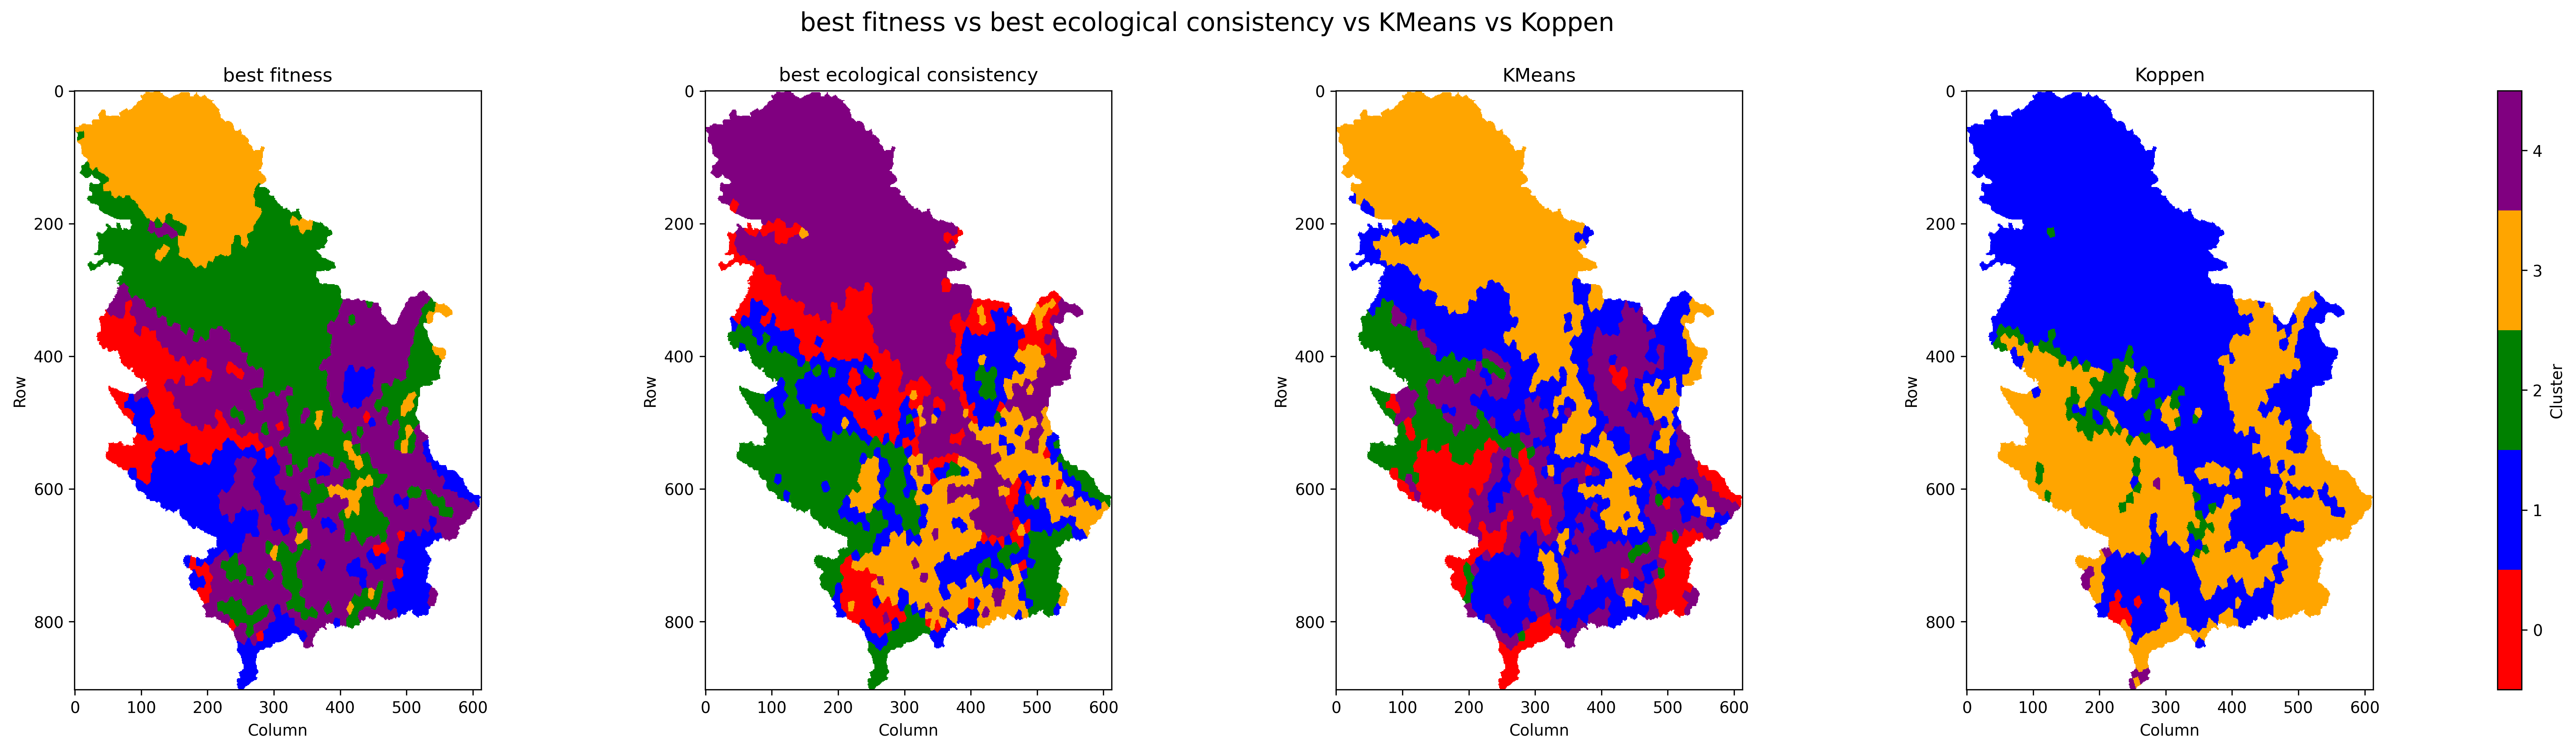
\includegraphics[width=\textwidth]{regionalization_comparison.png}
    \caption{Comparison of the best configuration according to fitness, the best configuration according to weighted ecological consistency, KMeans clustering and Köppen-Geiger classification.}
    \label{fig:regionalization_comparison}
\end{figure}

\begin{table}[ht]
\centering
\caption{Comparison of the selected regionalizations.}
\label{tab:regionalization_summary}
\begin{tabular}{lccc}
\hline
\textbf{Regionalization} & \textbf{Fitness} & \textbf{Weighted ecological consistency} & \textbf{ARI} \\
\hline
Köppen-Geiger & 0.3679 & 0.4426 & 0.3558 \\
KMeans & 0.2376 & 0.4744 & 1.0000 \\
Best fitness & 0.2325 & 0.4754 & 0.5431 \\
Best ecological consistency & 0.2633 & 0.4848 & 0.6211 \\
\hline
\end{tabular}
\end{table}

Several observations can be made from Figure~\ref{fig:regionalization_comparison}. The Köppen-Geiger classification produces relatively large and continuous climate regions with simple boundaries. In contrast, KMeans creates more fragmented regions because it groups locations only according to the climate variables.

The two ACO solutions show a different regionalization from both Köppen and KMeans. Large-scale climate regions are still recognizable, but many regional boundaries change. The best fitness and best ecological solutions are also visibly different from each other, even though both belong to the centroid-based family of algorithms.

The numerical results agree with these observations. The best fitness configuration achieves the lowest fitness value of all compared regionalizations. The best ecological configuration achieves the highest ecological consistency, while maintaining a fitness value that is still close to the optimum. Both ACO solutions also achieve higher ecological consistency than the Köppen-Geiger classification, while the best ecological solution slightly improves upon the KMeans baseline.

Overall, the visual comparison shows that the proposed optimization framework produces climate regionalizations that differ from both reference methods while maintaining competitive values for the optimization objective and ecological consistency.

\section{Future work}
\label{sec:future}

This project currently provides a framework for climate regionalization using Ant Colony Optimization. Several directions for future work could follow.

One future direction is to test the sensitivity to the number of clusters. In this work, the number of clusters is fixed to five, based on the number of dominant Köppen-Geiger classes after aggregation. Future experiments could compare results for other values, such as $K=4$, $K=6$ and $K=7$. This would show whether the fitness value and ecological consistency depend strongly on the chosen number of regions.

The ecological consistency measure developed in this work could also be incorporated directly into the optimization process. Instead of using it only for evaluation, future work could formulate climate regionalization as a multi-objective optimization problem. In that case, fitness and ecological consistency would be treated as separate objectives. This could produce a Pareto front of possible regionalizations instead of selecting only one best solution.

Another possible improvement is the development of pheromone update mechanisms that are invariant to cluster label permutations. In the current implementation, pheromone is associated with explicit cluster labels. Future work could investigate representations that reinforce equivalent clusterings regardless of the numerical labels assigned to the clusters.

Finally, the proposed validation methodology could be extended by including additional independent datasets. Besides vegetation, future studies could investigate the use of elevation, soil characteristics or other environmental variables that are influenced by climate. This would provide a more complete assessment of the obtained climate regionalizations.

\section{Conclusions}

This project investigated the use of Ant Colony Optimization (ACO) for climate regionalization of Serbia. The main goal was to develop a flexible optimization framework capable of producing alternative climate regionalizations and to evaluate them using any measure we choose.

A complete processing pipeline was developed, starting from raw climate raster layers and ending with the final climate regionalizations. The pipeline includes data preparation, graph construction, multiple ACO construction strategies, different pheromone update mechanisms and a validation framework based on land cover consistency. The modular implementation also allows new algorithms, heuristics and evaluation methods to be incorporated with relatively small modifications.

Several ACO variants were compared during the experimental evaluation. The results showed that the choice of construction strategy has the largest influence on the final solution. Centroid-based algorithms consistently achieved the best results, while graph and cohesion based approaches produced lower optimization quality and ecological consistency. Among the tested parameters, the heuristic weight ($\beta$) had the strongest influence, whereas the evaporation rate had only a small effect on the final regionalizations.

The experiment was also repeated using raw climate variables and PCA features. The broad ranking of construction strategies remained stable across feature representations: centroid-based methods were still strongest. This indicates that the conclusion is not only an artifact of the Köppen-inspired feature set. At the same time, the conclusion remains tied to the current fitness function, because its compactness term is centroid-based.

An important contribution of this work is the proposed ecological consistency metric based on the CORINE Land Cover dataset. Unlike the optimization objective, which measures compactness and spatial properties of the obtained clusters, the ecological consistency score evaluates how well the climate regions correspond to an independent environmental dataset. The experiments showed that these two measures do not always identify the same best solutions. This demonstrates that external validation provides useful additional information when selecting the final climate regionalization.

The obtained regionalizations were also compared with the traditional Köppen-Geiger classification and the KMeans clustering algorithm. The proposed ACO framework produced solutions with better optimization quality than Köppen while also achieving higher ecological consistency. The best ecological ACO solution also slightly improved the ecological consistency of the KMeans baseline, demonstrating that the proposed optimization framework is capable of producing competitive climate regionalizations.

The multi-seed validation step showed that top configurations are close to each other. With five seeds, Wilcoxon signed-rank tests did not provide enough evidence to claim statistically significant differences among the top configurations. Therefore, the safest conclusion is at the level of strategy families rather than individual parameter settings.

Overall, the results show that Ant Colony Optimization is a suitable approach for climate regionalization. Although the centroid-based strategies proved to be the most effective within the tested framework, the developed methodology provides a flexible foundation for investigating alternative optimization objectives, construction strategies and validation methods in future research.


\begin{thebibliography}{99}

\bibitem{beck2018}
Beck, H. E., Zimmermann, N. E., McVicar, T. R., Vergopolan, N., Berg, A., and Wood, E. F. (2018).
Present and future Köppen-Geiger climate classification maps at 1-km resolution.
\textit{Scientific Data}, 5, 180214.
https://doi.org/10.1038/sdata.2018.214

\bibitem{carvalho2016}
Carvalho, M. J., Melo-Gonçalves, P., Teixeira, J. C., and Rocha, A. (2016).
Regionalization of Europe based on a K-Means Cluster Analysis of the climate change of temperatures and precipitation.
\textit{Physics and Chemistry of the Earth, Parts A/B/C}, 94, 22--28.
https://doi.org/10.1016/j.pce.2016.05.001

\bibitem{clcManual2021}
Copernicus Land Monitoring Service. (2021).
Product user manual: CORINE Land Cover from 1990 to 2018 and CORINE Land Cover Changes.
Version 1.0.

\bibitem{copernicusCLC2018}
Copernicus Land Monitoring Service. (2018).
CORINE Land Cover 2018, raster 100 m, Europe, 6-yearly.
https://doi.org/10.2909/960998c1-1870-4e82-8051-6485205ebbac

\bibitem{deneubourg1991}
Deneubourg, J.-L., Goss, S., Franks, N., Sendova-Franks, A., Detrain, C., and Chrétien, L. (1991).
The dynamics of collective sorting: robot-like ants and ant-like robots.
In \textit{Proceedings of the First International Conference on Simulation of Adaptive Behavior: From Animals to Animats}, 356--363.

\bibitem{dorigo1996}
Dorigo, M., Maniezzo, V., and Colorni, A. (1996).
Ant system: optimization by a colony of cooperating agents.
\textit{IEEE Transactions on Systems, Man, and Cybernetics, Part B: Cybernetics}, 26(1), 29--41.
https://doi.org/10.1109/3477.484436

\bibitem{dorigo2004}
Dorigo, M., and Stützle, T. (2004).
\textit{Ant Colony Optimization}.
MIT Press.

\bibitem{fovell1993}
Fovell, R. G., and Fovell, M.-Y. C. (1993).
Climate zones of the conterminous United States defined using cluster analysis.
\textit{Journal of Climate}, 6(11), 2103--2135.
https://doi.org/10.1175/1520-0442(1993)006<2103:CZOTCU>2.0.CO;2

\bibitem{gadm2022}
GADM. (2022).
GADM database of Global Administrative Areas, version 4.1.
https://gadm.org/

\bibitem{handl2006}
Handl, J., Knowles, J., and Dorigo, M. (2006).
Ant-based clustering and topographic mapping.
\textit{Artificial Life}, 12(1), 35--61.
https://doi.org/10.1162/106454606775186400

\bibitem{hubert1985}
Hubert, L., and Arabie, P. (1985).
Comparing partitions.
\textit{Journal of Classification}, 2, 193--218.
https://doi.org/10.1007/BF01908075

\bibitem{liu2012}
Liu, X., Lao, C., Li, X., Liu, Y., and Chen, Y. (2012).
An integrated approach of remote sensing, GIS and swarm intelligence for zoning protected ecological areas.
\textit{Landscape Ecology}, 27, 447--463.
https://doi.org/10.1007/s10980-011-9684-1

\bibitem{koppen1936}
Köppen, W. (1936).
Das geographische System der Klimate.
In W. Köppen and R. Geiger (Eds.), \textit{Handbuch der Klimatologie}, Band 1, Teil C.
Gebrüder Borntraeger.

\bibitem{milovanovic2017}
Milovanović, B., Ducić, V., Radovanović, M., and Milivojević, M. (2017).
Climate regionalization of Serbia according to Köppen climate classification.
\textit{Journal of the Geographical Institute ``Jovan Cvijić'' SASA}, 67(2), 103--114.
https://doi.org/10.2298/IJGI1702103M

\bibitem{peel2007}
Peel, M. C., Finlayson, B. L., and McMahon, T. A. (2007).
Updated world map of the Köppen-Geiger climate classification.
\textit{Hydrology and Earth System Sciences}, 11, 1633--1644.
https://doi.org/10.5194/hess-11-1633-2007

\bibitem{peng2019}
Peng, J., Zhao, S., Dong, J., Liu, Y., Meersmans, J., Li, H., and Wu, J. (2019).
Applying ant colony algorithm to identify ecological security patterns in megacities.
\textit{Environmental Modelling \& Software}, 117, 214--222.
https://doi.org/10.1016/j.envsoft.2019.03.017

\bibitem{sheridan2011}
Sheridan, S. C., and Lee, C. C. (2011).
The self-organizing map in synoptic climatological research.
\textit{Progress in Physical Geography}, 35(1), 109--119.
https://doi.org/10.1177/0309133310397582

\bibitem{swenson2019}
Swenson, L. M., and Grotjahn, R. (2019).
Using self-organizing maps to identify coherent CONUS precipitation regions.
\textit{Journal of Climate}, 32(22), 7747--7761.
https://doi.org/10.1175/JCLI-D-19-0352.1

\bibitem{tong2024}
Tong, Z., Yang, J., Liu, Y., Zhang, Z., Liu, S., Lu, Y., Pang, B., and An, R. (2024).
Cooling and optimizing urban heat island based on a thermal knowledge-informed multi-type ant colony model.
\textit{Remote Sensing of Environment}, 306, 114138.
https://doi.org/10.1016/j.rse.2024.114138

\bibitem{zhang2021}
Zhang, Y., Chen, X., Lv, D., and Zhang, Y. (2021).
Optimization of urban heat effect mitigation based on multi-type ant colony algorithm.
\textit{Applied Soft Computing}, 112, 107758.
https://doi.org/10.1016/j.asoc.2021.107758

\end{thebibliography}

\end{document}
